\documentclass[../main.tex]{subfiles}
\graphicspath{{./images/}}
%%%%%%%%%%%%%%%%%%%%%%%%%%%%%%%%%%%%%%%%%%%%%%%%%%%%%%%%%%%%%%%%%

\begin{document}


\section{3D approach to object detection} \label{sec:3D_approach}
3D approach introduction goes here.

\subsection{Filtering}
Filtering point cloud data is in some sense equivalent to the 2D curation of the dataset, with its particularities. In general, data coming from depth sensors of any kind tends to have noise in the measurements, specially for distances that match the working range of the cameras. Hence, it is very important to filter out said noise as much as possible to ease further processing an increment the chances of success. There are many filtering techniques, and PCL offers a lot of variety in this regard. For this work, however, only 2 basic filtering techniques have been applied, and work well enough for the project. The first technique is a \emph{conditional filter} and the second one, applied in chain after it, is the \emph{statistical filter}. This section will explain how they work from a theoretical point of view and provide samples from the testbench to compare the `before' and `after' applying them.

\paragraph{The Conditional Filter}
As the name implies the conditional filter discerns inliers from outliers by establishing a condition. Said condition is defined as being inside a distance $R$ from the origin of coordinates (generally the sensor of the camera). In other words, a sphere of radius $R$ is centered in the origin of coordinates and all points falling inside are considered as inliers, while those outside are considered outliers. The advantage of this simple method is twofold: on the one hand, points too far tend to not be of interest, since they belong to the walls of the room in which the testbench is placed. On the other, even if points far away are of interest they will likely be too noisy, and may not even be worthy to keep them. See figure \ref{fig:conditional_filter_testbench} for an example on the testbench. The main disadvantage of the conditional filter is that the distance $R$, or at least an approximation of it, needs to be known beforehand. For cases where the camera may be aiming at the testbench in a range of distances (not contemplated in this work) $R$ should be big enough to accommodate said range or otherwise valuable points will be deleted.

\begin{figure}[htbp]
    \centering
    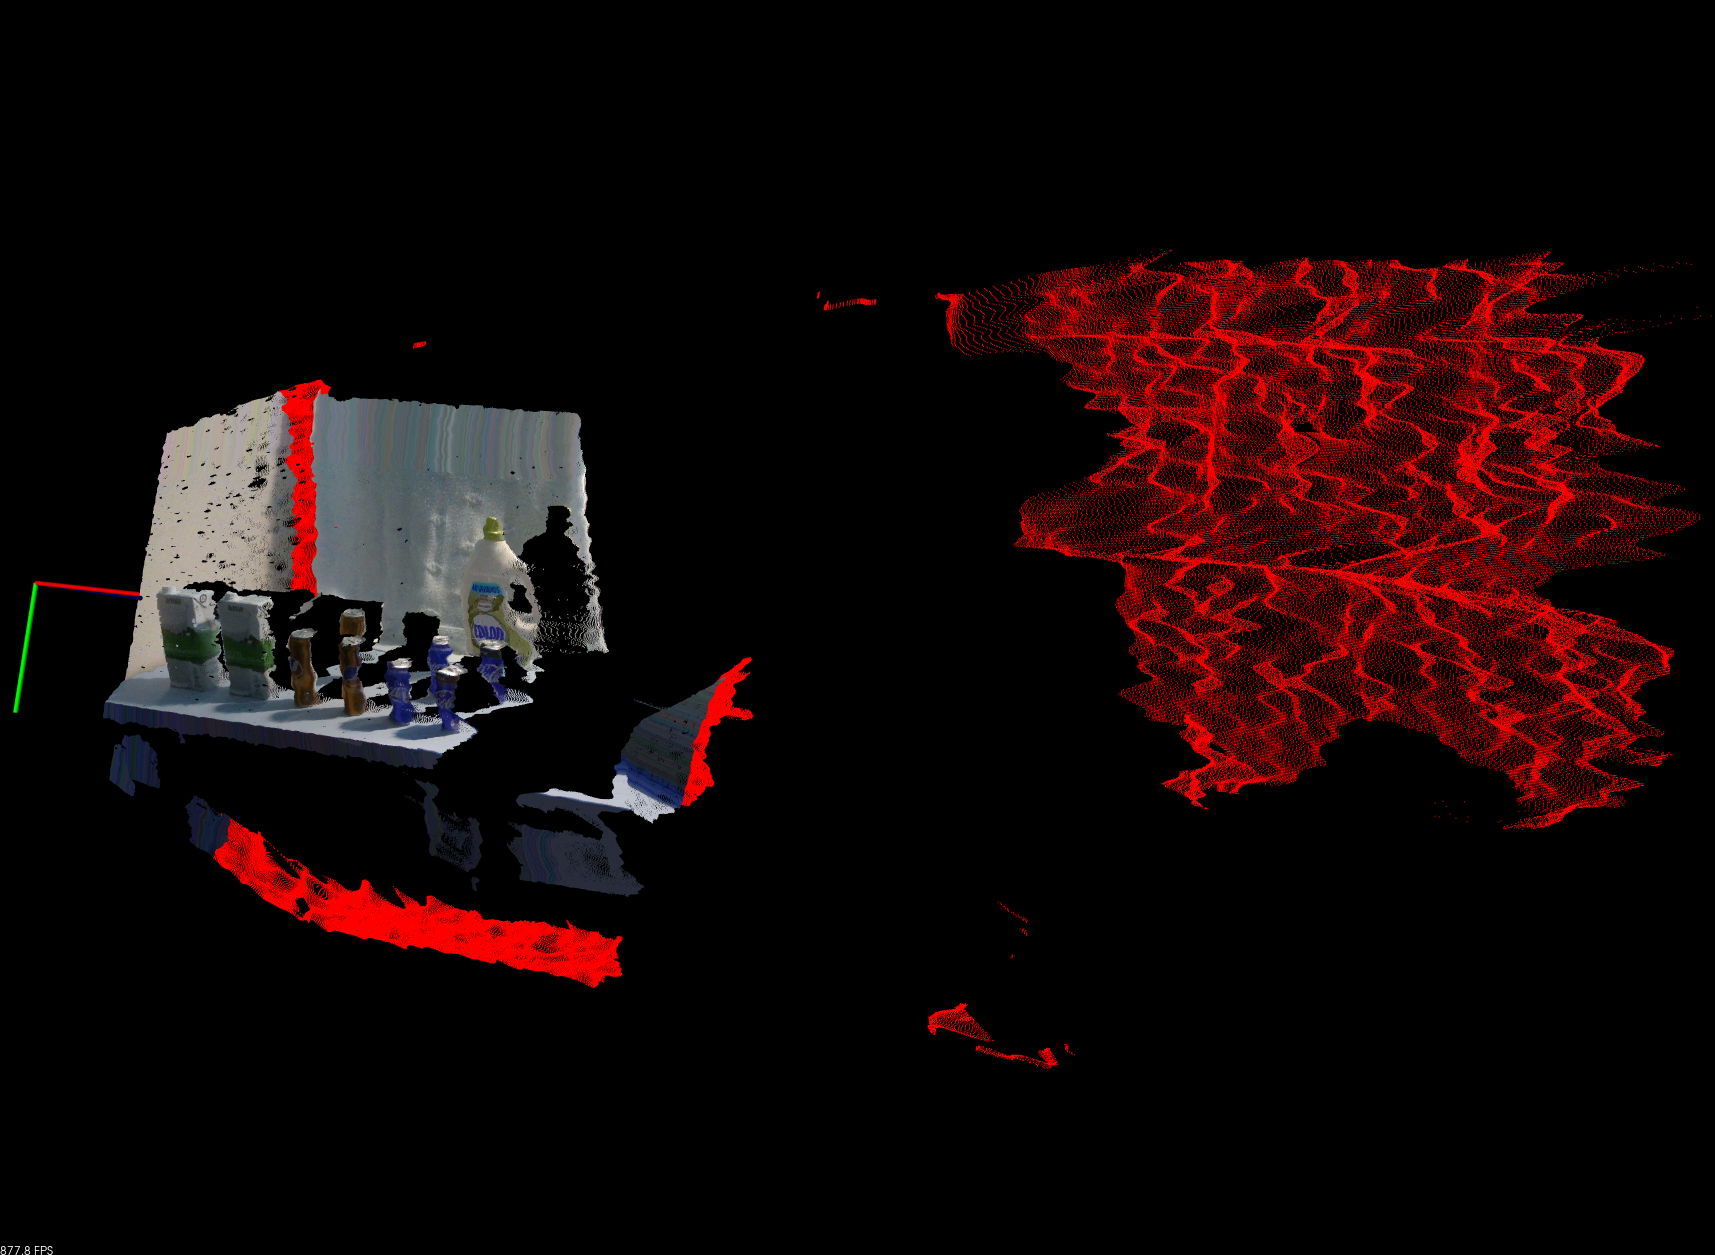
\includegraphics[width=1\textwidth]{images/conditional_filter_testbench.png}
    \caption{Conditional filter with $R=1.2$ meters. As it can be observed, points that belong to other things (mainly the wall of the room) beyond the testbench are deleted, marked in red. Note: disregard the fact that the RGB channels have been flipped to BGR.}
    \label{fig:conditional_filter_testbench}
\end{figure}

\paragraph{The Statistical Filter}
The statistical filter, implemented in PCL as \emph{statistical outlier removal}, aims to eliminate isolated pixels by fitting a Gaussian distribution over the mean distance between points, called $\mu_{d}$. A multiplier of standard deviations $\sigma_{d}$ (a value established by the user) from the mean $\mu_{d}$ acts as threshold, indicating that points having a mean distance to other points that is $\sigma_{d}$ times the standard deviation of the mean need to be removed. Note that ``the mean distance of a point to other points'' is not actually computed for every single other point, but rather a subset of closest neighbors $n_{k}$ large enough to be meaningful. For the point clouds obtained of the testbench $n_{k}=50$ has been found to work well enough. The algorithm is detailed below, and graphically exemplified in figure \ref{fig:stat_filter_diagram}.

\begin{enumerate}
    \item The user defines the number of closest points $n_{k}$ to be evaluated at every point $P_{i}$, and the multiplier $\sigma_{d}$ of standard deviations from the mean distance.
    \item For every point $P_{i}$ in the point cloud do:
    \begin{enumerate}
        \item Get the index of the $n_{k}$ closest points to $P_{i}$.
        \item Compute the average distance $d_{i}$ of said points.
    \end{enumerate}
    \item Compute the mean distance $\mu_{d}$ of all distances $d_{i}$.
    \item Compute the standard deviation $\sigma_{d}$.
    \item Compute the threshold like $T=\mu_{d} + \alpha \cdot \sigma_{d}$
    \item Remove all points having a mean distance $d_{i} > T$.
\end{enumerate}

The statistical filter has been very useful to eliminate sparse noise in the edges of objects, as it can be seen in figure \ref{fig:stat_filtered_compareStds} behind the detergent.

\begin{figure}[htbp]
    \centering
    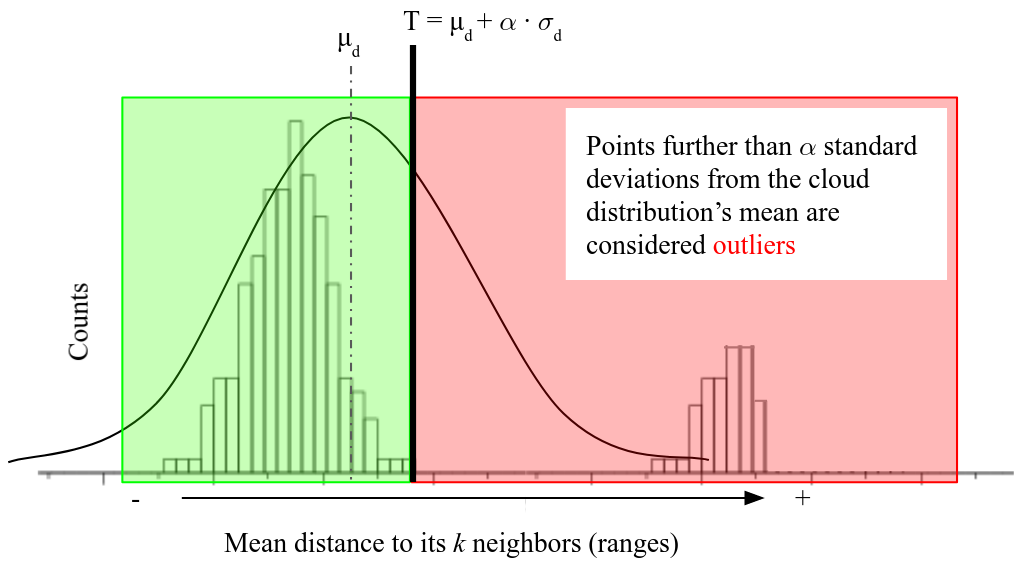
\includegraphics[width=0.9\textwidth]{images/stat_filter_diagram.png}
    \caption{What the statistical outlier removal does explained in a single figure.}
    \label{fig:stat_filter_diagram}
\end{figure}

\begin{figure}[htbp]
    \centering
    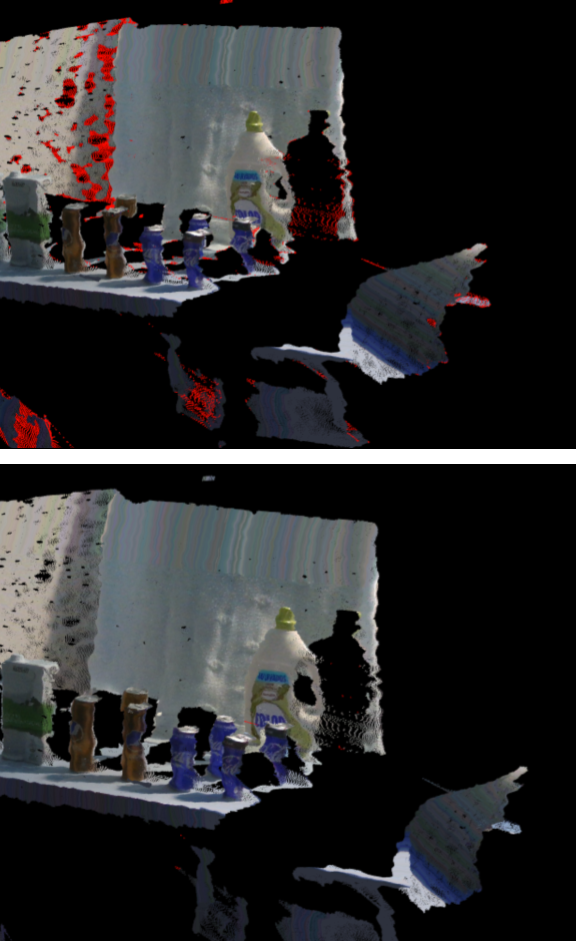
\includegraphics[width=0.7\textwidth]{images/stat_filtered_compareStds.png}
    \caption{Comparison of different standard deviation multipliers $\sigma$. \emph{Up}: $\sigma=0.25$. \emph{Down}: $\sigma=3$. These images are a zoom in of figures \ref{fig:stat_filter025std} and \ref{fig:stat_filter3std}.}
    \label{fig:stat_filtered_compareStds}
\end{figure}

\begin{figure}[htbp]
    \centering
    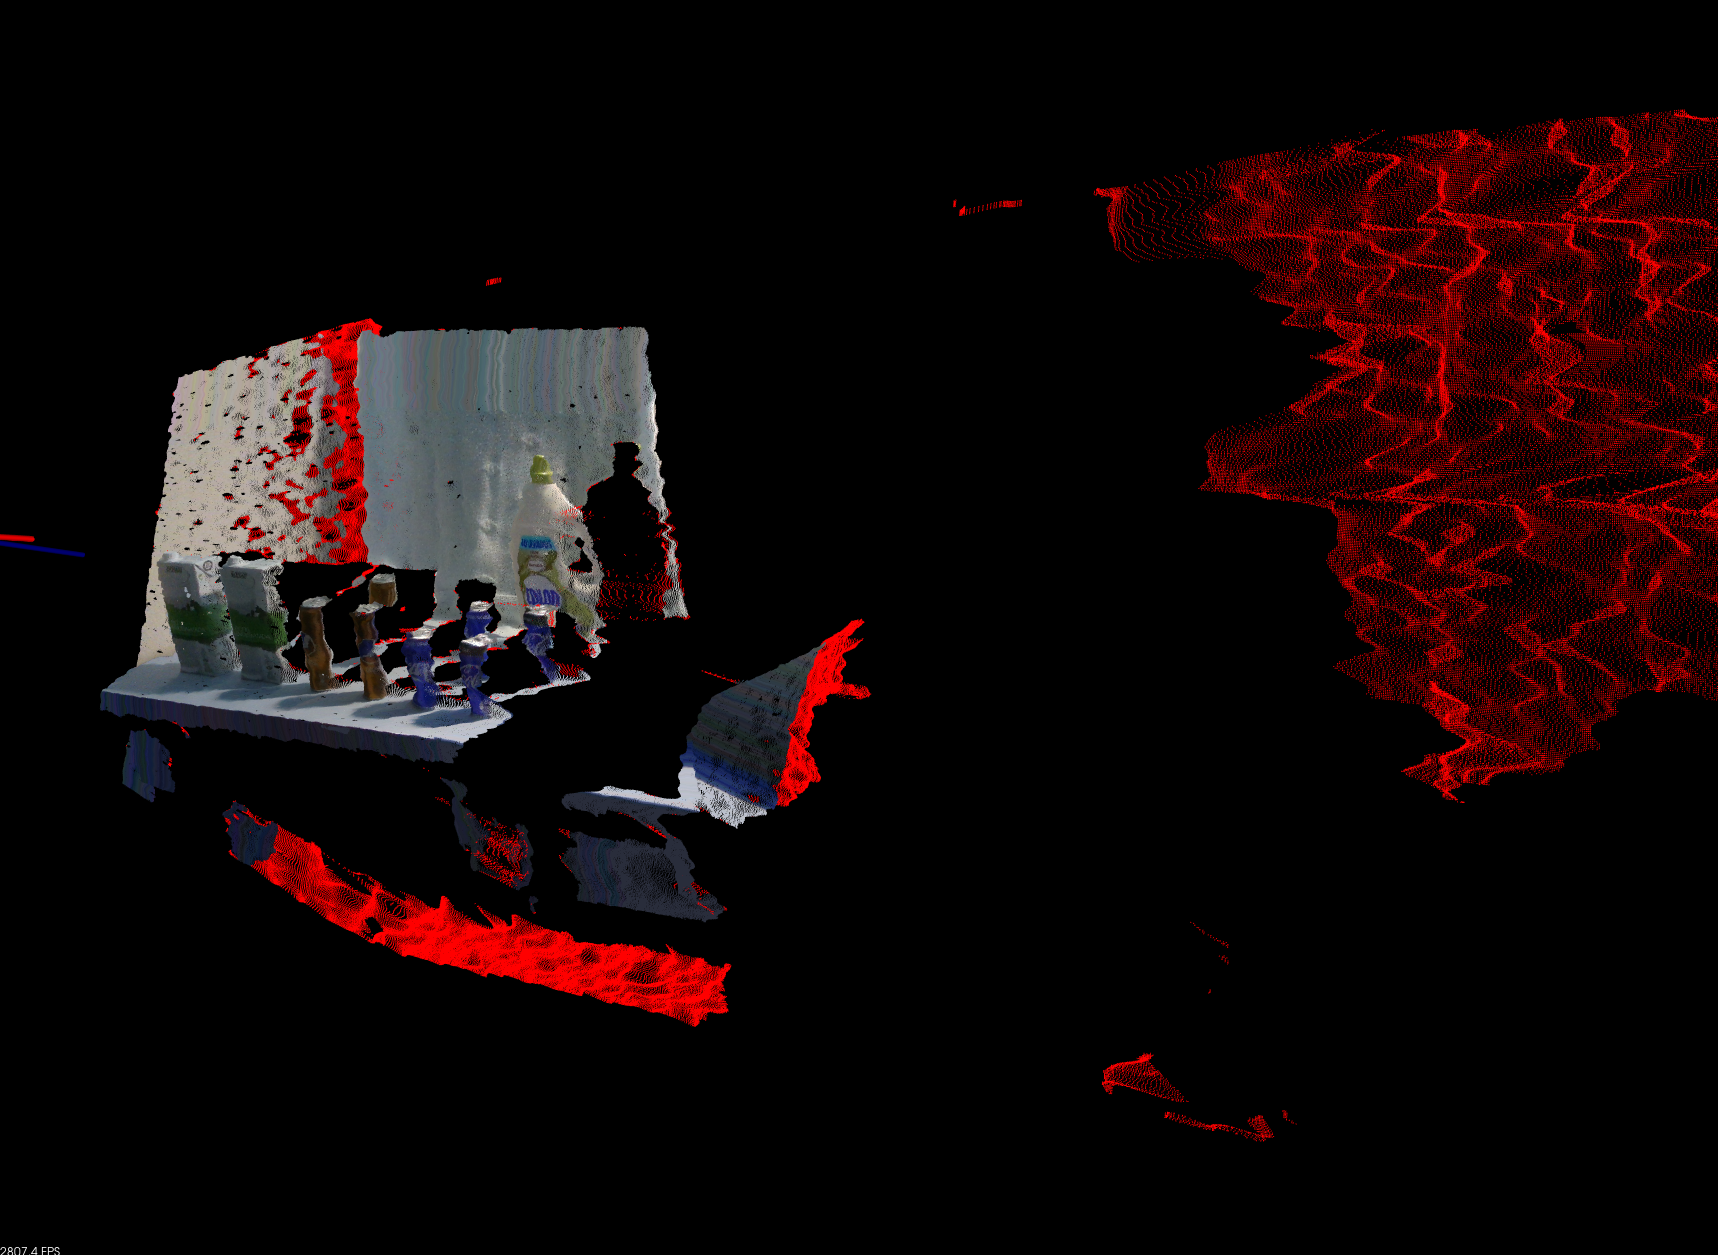
\includegraphics[width=1\textwidth]{images/conditional_stat_filter_testbench.png}
    \caption{Result of applying the conditional filter with $R=1.2$ meters, first, and then the statistical filter with $\alpha=1$ and $n_{k}=50$. As it can be observed, some dispersed, non-dense and isolated points like the ones behind the detergent and some cans have been removed (marked in red).}
    \label{fig:conditional_stat_filter_testbench}
\end{figure}

\begin{figure}[htbp]
    \centering
    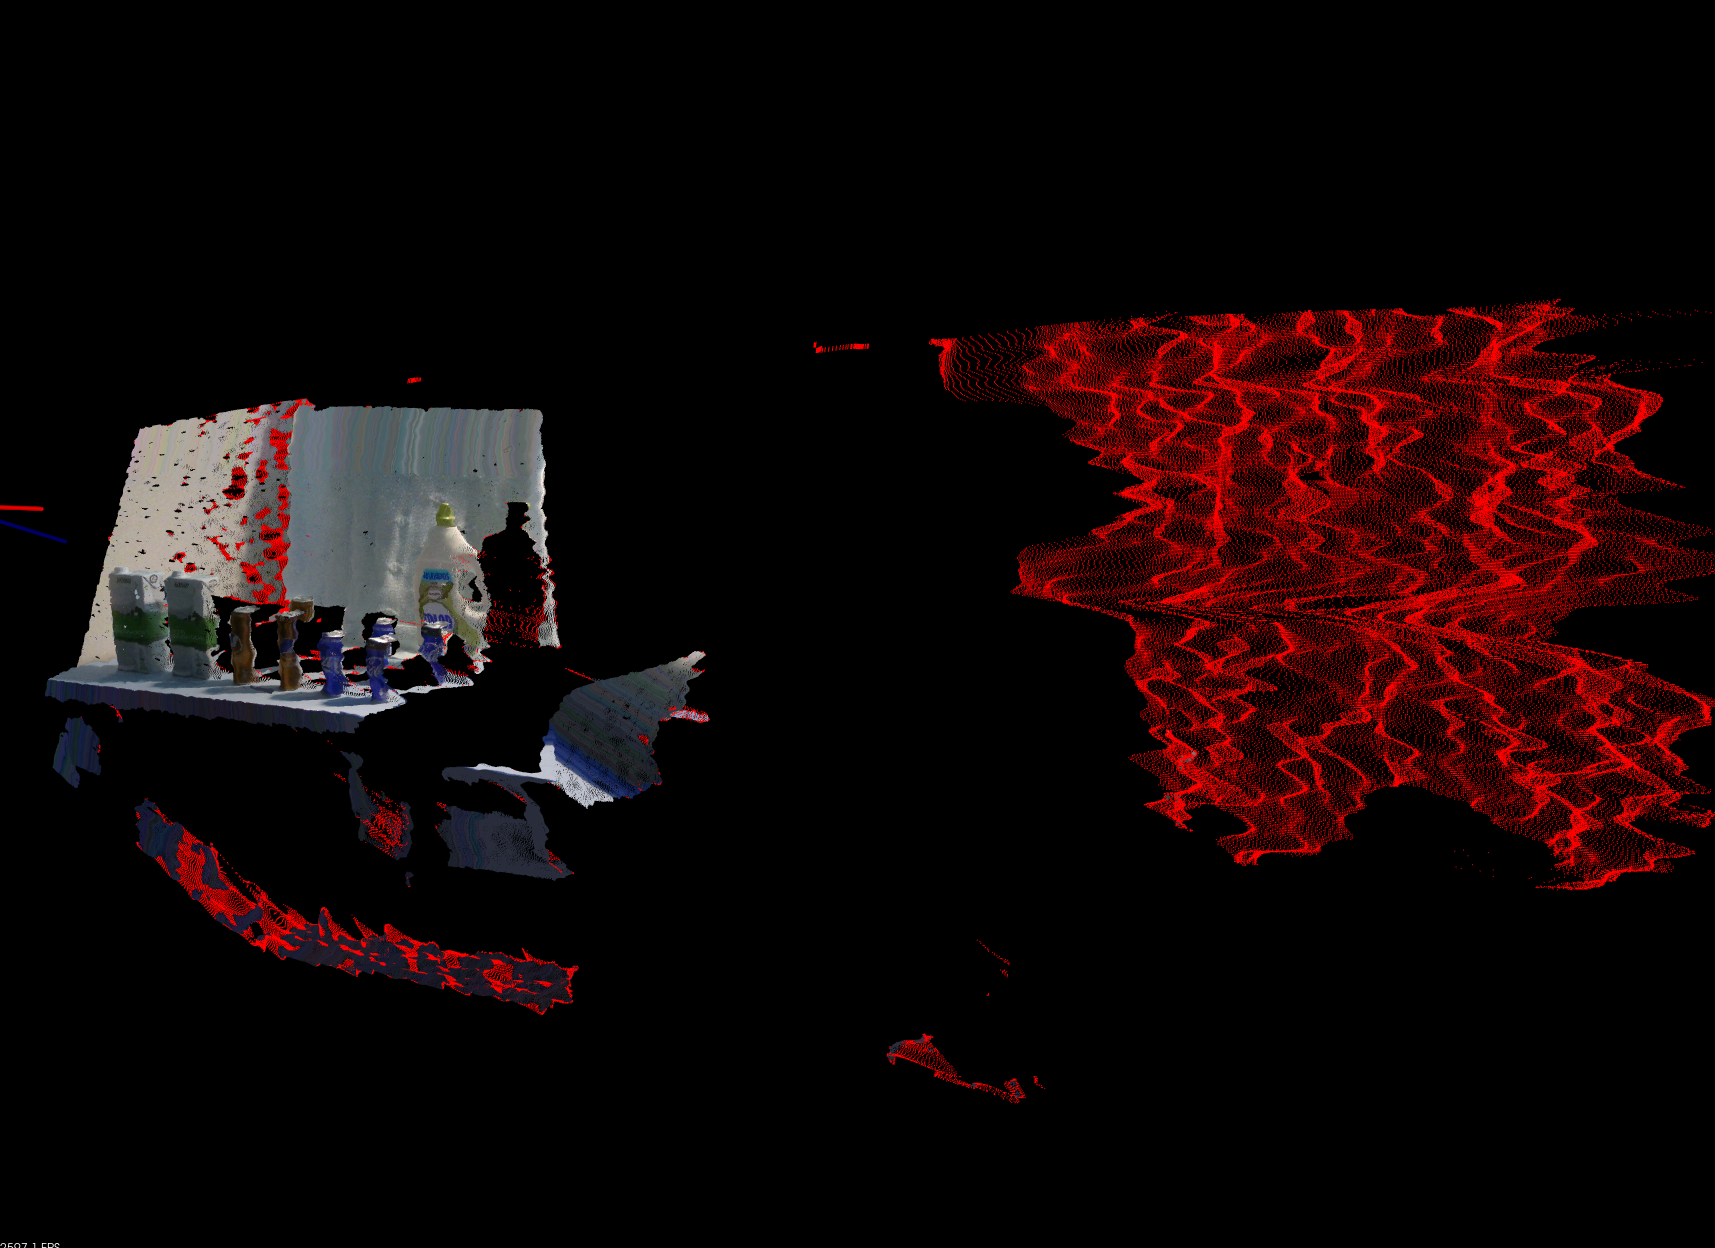
\includegraphics[width=1\textwidth]{images/stat_filter025std.png}
    \caption{Result of applying the statistical filter with $\alpha=0.25$ and $n_{k}=50$. As it can be observed, even the wall was removed due the sparsity of the points caused by the large noise at those distances.}
    \label{fig:stat_filter025std}
\end{figure}

\begin{figure}[htbp]
    \centering
    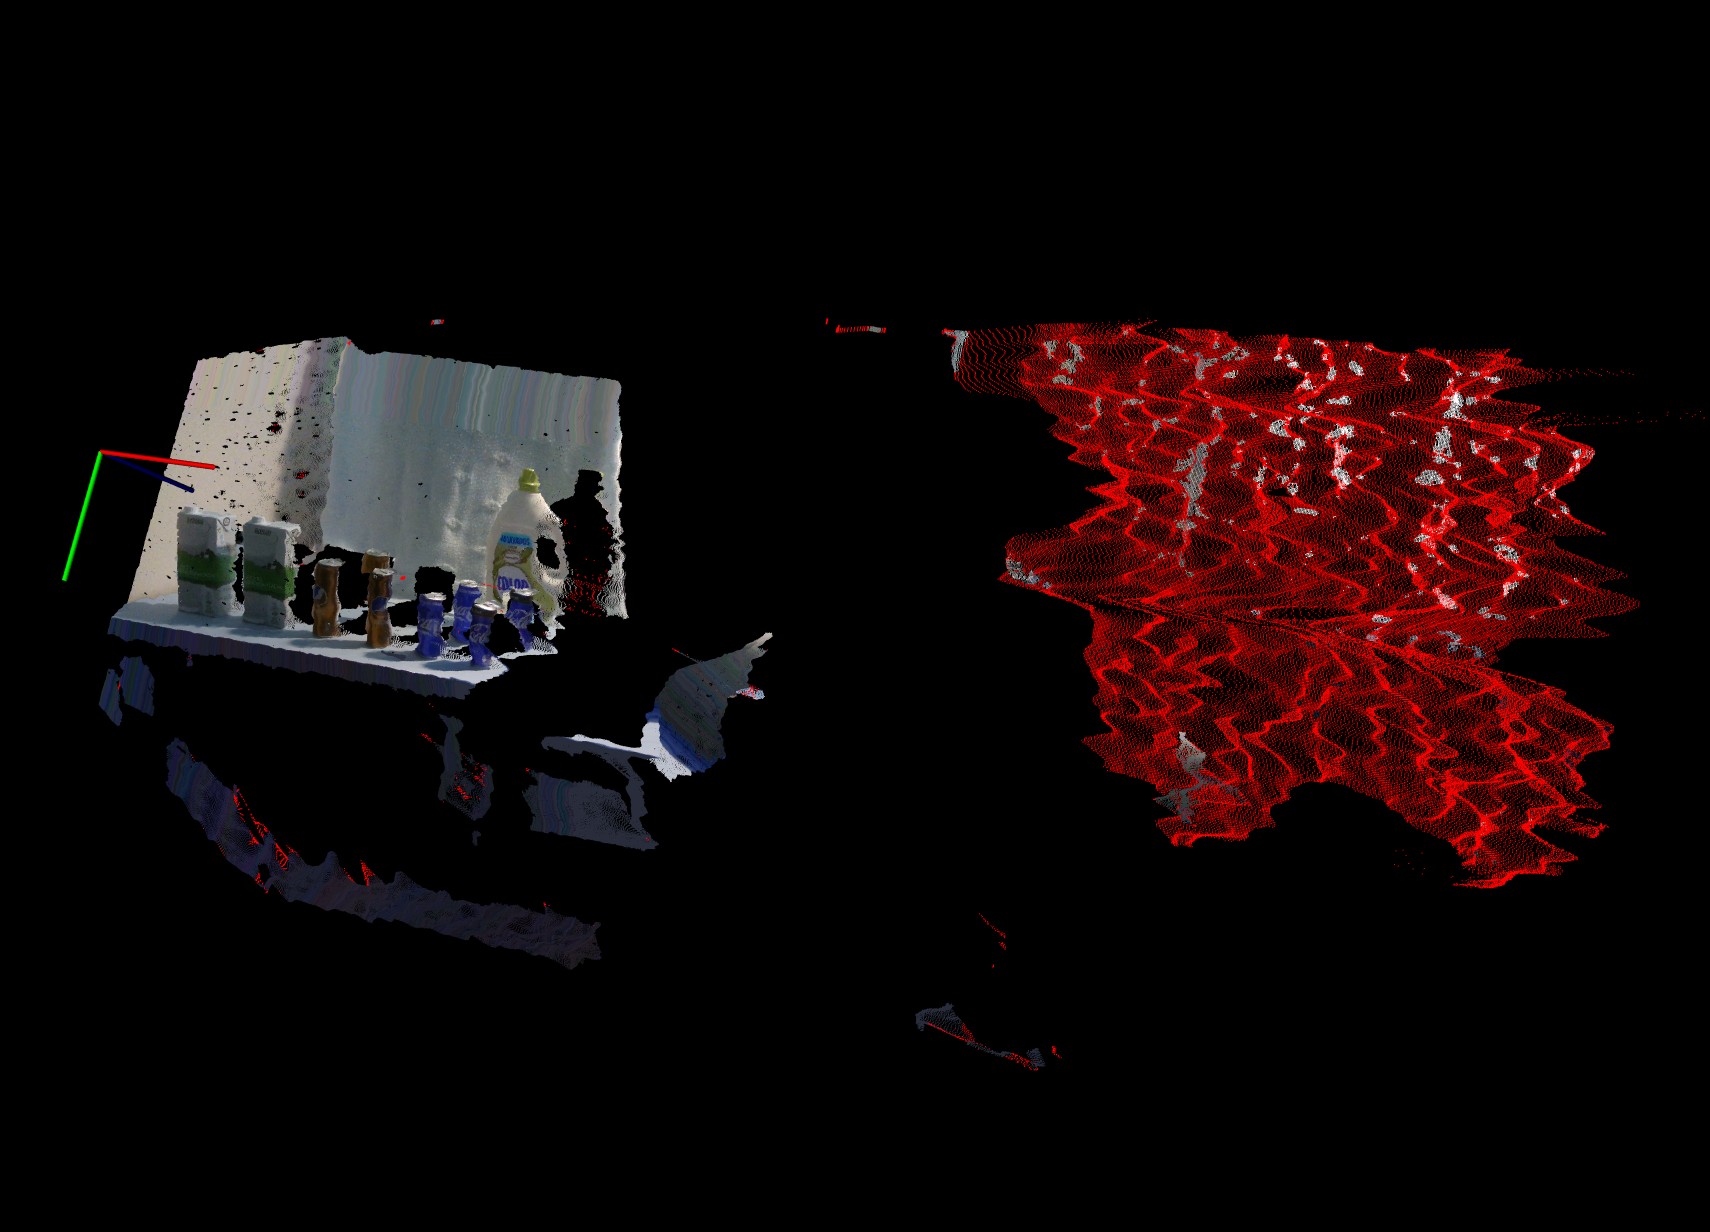
\includegraphics[width=1\textwidth]{images/stat_filter1std.png}
    \caption{Result of applying the statistical filter with $\alpha=1$ and $n_{k}=50$. As it can be observed, since the multiplier $\sigma$ is larger, the most dense point.}
    \label{fig:stat_filter1std}
\end{figure}

\begin{figure}[htbp]
    \centering
    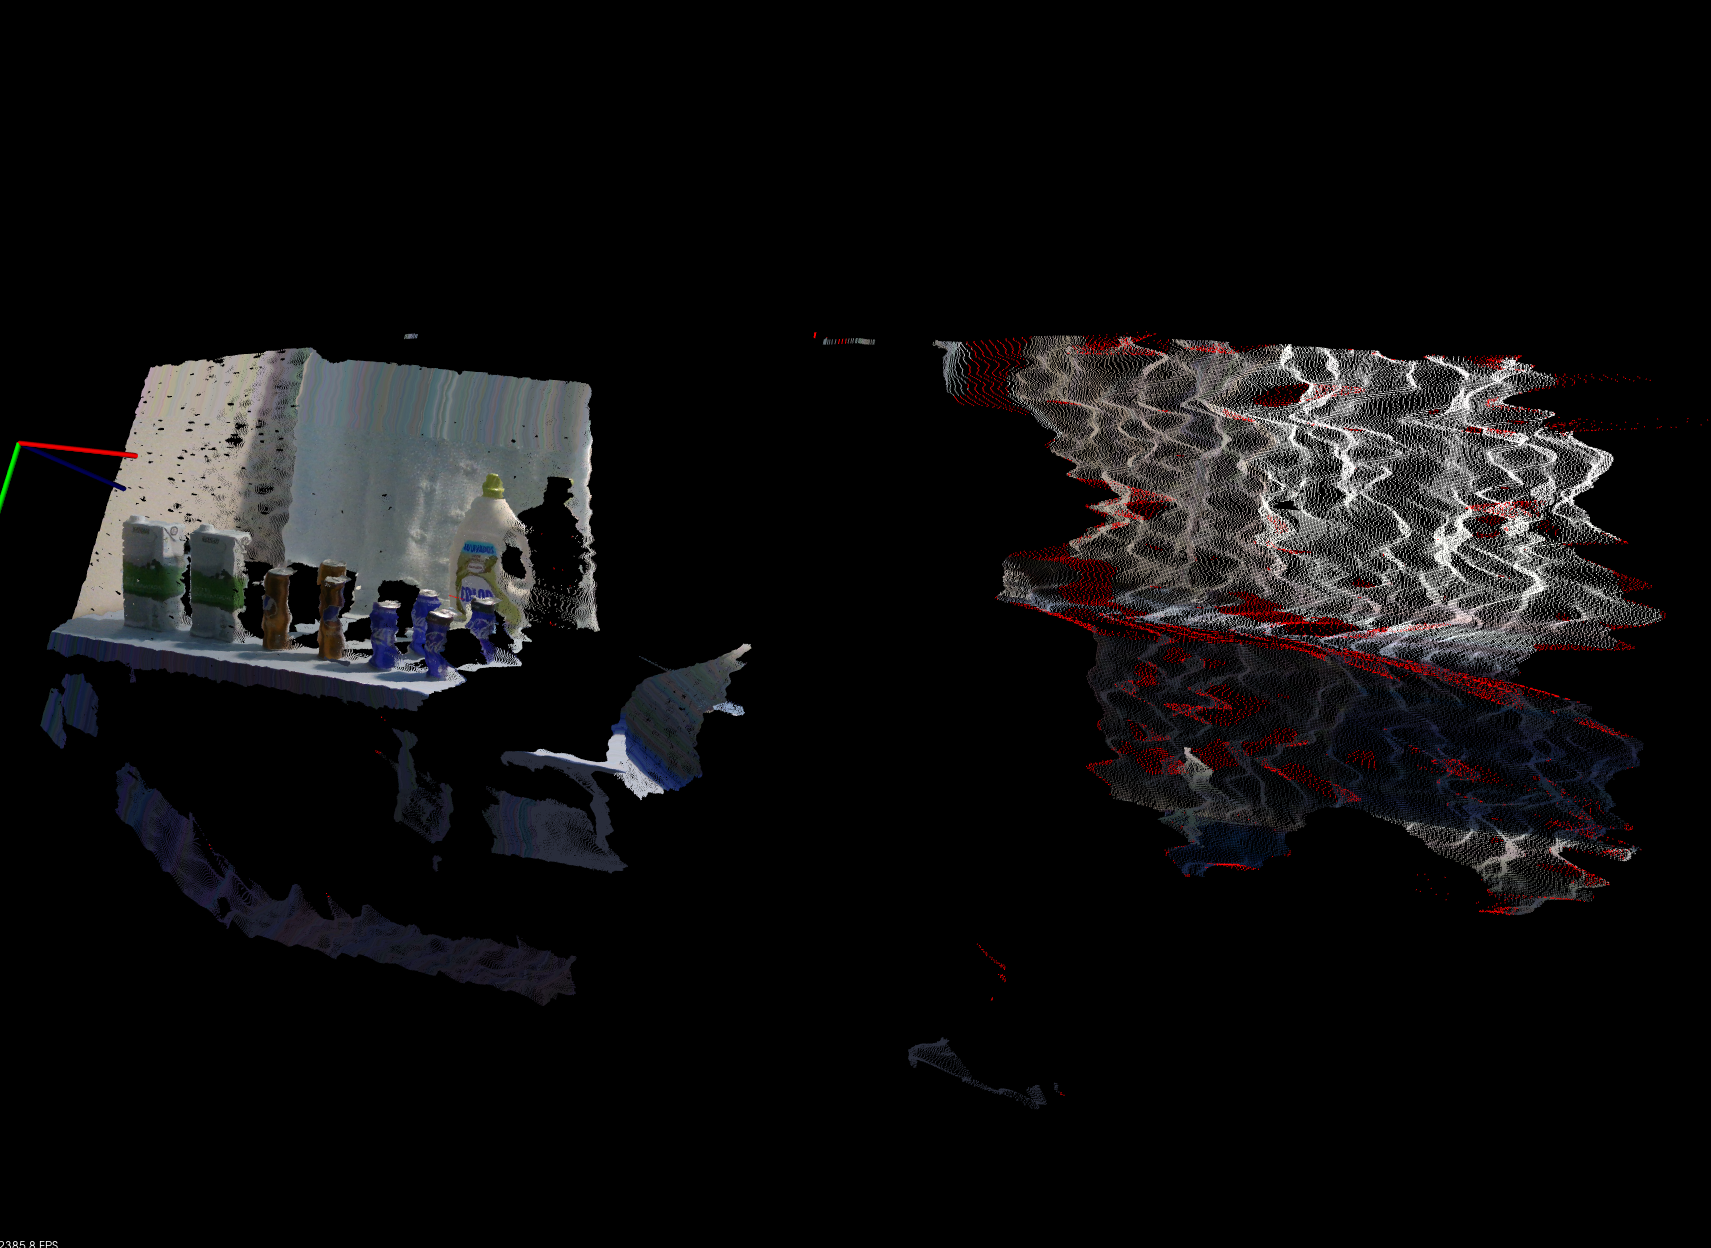
\includegraphics[width=1\textwidth]{images/stat_filter3std.png}
    \caption{Result of applying the statistical filter with $\alpha=3$ and $n_{k}=50$. As it can be observed, $\sigma$ is so large that very little point are removed.}
    \label{fig:stat_filter3std}
\end{figure}


\subsection{Registration}
In the jargon, the concept \emph{registration} refers to the act of composing into one single point cloud of several distinct but similar point clouds of one same scene, all taken from different viewpoints. Registration may also be referred to as \emph{mapping}.

Depth images can only measure the distance of those points facing the camera's position, so point clouds that aim to integrate the complex shapes of certain objects need to incorporate information from different viewpoints. Registration is also needed to create complex maps of large regions. Hence the need to compose different point clouds into one. This, however, is not a trivial thing to do: every point cloud (created from a depth image taken by the camera) is different, and the registration algorithm, whatever that may be, needs to account for that and still be able to find enough similarities between them so as to properly couple them together.

Registration is not applied to all clouds at the same time, but rather by pairs. For instance, if 5 depth images are taken with successive captures, one with the camera slightly moved from the other, and for each a point cloud is created, the registration algorithm is applied incrementally by pairs. That is, the output algorithm after registration is the input cloud for the next registration, alongside the new point cloud to be registered, and so on until the list of point clouds is exhausted. From now on, the source cloud that needs to be aligned will be called X, and the target cloud to which X is aligned will be called Y.

A registration algorithm, of any kind, needs two things: (1) correspondences between the points in target Y and source X and (2) the parameters of the transformation that best aligns those corresponding data points. The unknown point association defined in (1) may be tackled with a wide range of algorithms, but the most standard one, and the one used in this thesis, is the \emph{Iterative Closest Point} (ICP) algorithm \cite{icp_chen}, \cite{icp_besl}. As it will be explained later, ICP works around the idea that no optimal point correspondences can be found, and hence there's the need to iteratively find correspondences and alignments until a convergence is reached. In (2) the transformation that best aligns the corresponding data points (whichever that correspondence is in the sequence of ICP iterations) is tackled by finding the translation vector $t$ and the rotation matrix $R$ to be applied to cloud X so that it is optimally aligned with target cloud Y. Good news is that there exists an optimal closed-form solution that does not require an initial guess nor any iteration. In the following paragraphs the ICP algorithm is going to be explained in more detail.

\paragraph{Unknown data association: source and target point cloud correspondences}
As mentioned, the goal given a source cloud X and a target cloud Y is to align X to Y in the most optimal manner. As it will be explained later, the alignment between two sets of points has a closed-form solution, provided that there is a one-to-one correspondence of the points in both clouds. The issue here is to do a \emph{good enough} matching of points for X and Y so as to have some success in the posterior alignment step. An example of this can be seen in figure \ref{fig:icp_demo}. 

\begin{figure}[htbp]
    \centering
    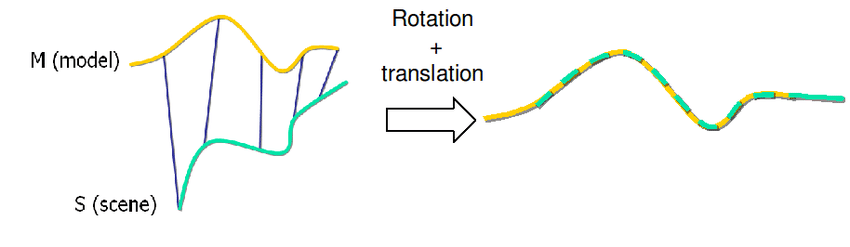
\includegraphics[width=0.8\textwidth]{images/icp_demo.png}
    \caption{The data association process: source cloud X has its points matched to target cloud Y (although 2D in this case), so that an alignment step can take place. This is repeated until convergence. Image extracted from \cite{icp_demo_figure}.}
    \label{fig:icp_demo}
\end{figure}

The data association set is then repeated and the alignment computed again. If its value converges, the ICP stops. If it doesn't, it keeps on iterating. See the algorithm sketch in \ref{lst:icp_algo}. As one could guess, this process is very prone to error due to local minima. Hence it is imperative that, no matter what data association method is used, the points be ``somehow" pre-aligned before starting the ICP. This ``somehow" can't really be measured, and will vary from cloud to cloud. The lemma is that they need to be somewhat close enough. For systems that integrate Inertia Measurement Units or other kind of positional measurements this is not a problem, since the position and orientation at every point cloud is known. This makes the alignment from one point cloud to another a matter of applying a rotation and a translation, leaving the ICP for mere refinement. Point clouds that do not have positional information may rely on computing descriptors and matching them so as to have a broad alignment prior to the ICP. This thesis does not work this assumption, however. To remediate this, all sequences of images taken from the testbench are performed by subtly moving the camera in short increments of distance, and performing the ICP by pairs in the same order the clouds were taken. This way the distance from cloud to cloud is never too large and hence good enough to start the ICP with chances of success\footnote{If there is no initial pre-alignment one could align the center of masses of both point sets before the data association.}.

\begin{algorithm}[H]
    \SetAlgoLined
    $\overline{x}=x_{e}$\\
    error $e=\infty$\\
    \While{$e$ has decreased and $e$ $<$ threshold}{
        C=\texttt{find\_correspondences\_between\_points(\{$y_{n}, \overline{x}_{n}$\})}\\
        $t, R$=\texttt{compute\_alignment(C)}\\
        $\overline{x}_{n} = R(x_{n} - x_{0} + y_{0})$\\
        $e = E(t, R)$\\
    }
    return \{$\overline{x}_{n}$\}\\
    \caption{The standard ICP algorithm}
    \label{lst:icp_algo}
\end{algorithm}

A main question remains: how is the data association actually performed. The vanilla method is by subsampling uniformly both the target and source clouds, and computing the closest neighbor for every point between X and Y. There are, however, other methods besides subsampling and the closest distance that may work best for some applications. With respect to the type of sampling, there are some notable alternatives:
\begin{itemize}
    \item Random sampling. Points in the space are sampled randomly for both clouds X and Y. See figure \ref{fig:normal_sampling_icp} image (a) for an example.
    \item Feature-based sampling. By computing descriptor vectors of both clouds and matching them (that is, matching their features).
    \item Normal-based sampling. Ensures that samples have a uniform distribution of their normals. In other words, points are sampled in the normal space. This is specially useful for smooth areas with occasional features (see \ref{fig:normal_sampling_icp}).
\end{itemize}
\begin{figure}[htbp]
    \centering
    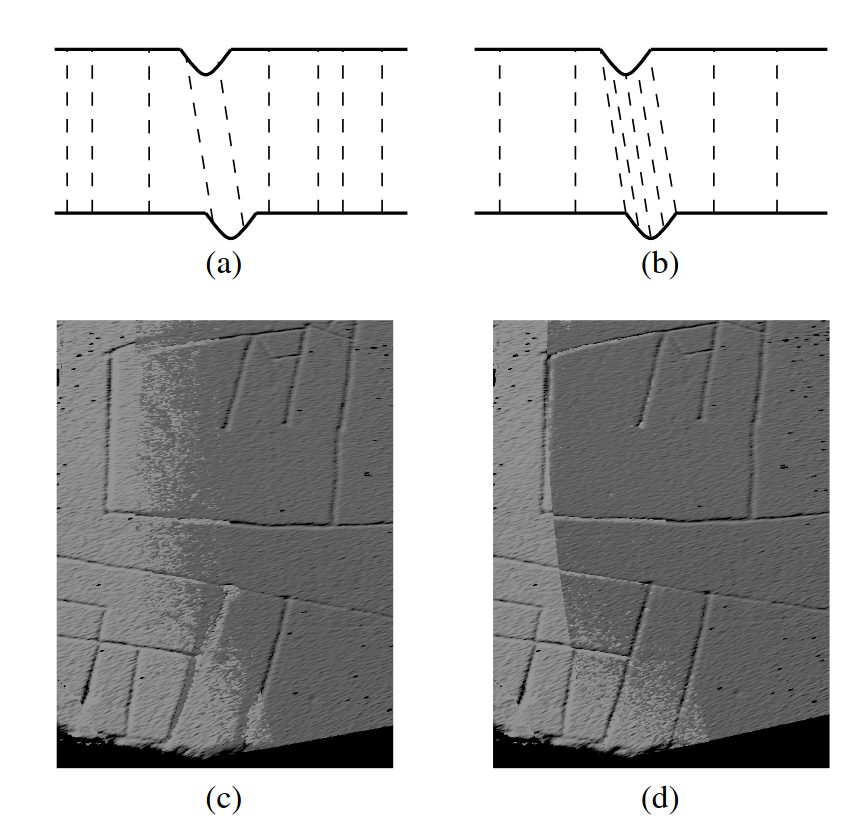
\includegraphics[width=0.8\textwidth]{images/normal_sampling_icp.png}
    \caption{(a) Pairs of points found by random sampling (uniform sampling would look the same but the correspondence lines would be evenly separated) and (b) points sampled by normal space sampling. Since normals need to be uniformly sampled, the slope of the notch is sampled more compared to (a). This yields different reconstructions, shown below. As it can be observed, when the surface is mostly smooth but has occasional features normal sampling works best to help converge to alignment. Image extracted from \cite{rusinkiewicz2001efficient_icps}.}
    \label{fig:normal_sampling_icp}
\end{figure}

Regarding the data association technique, there are also some alternatives besides closest distance:
\begin{itemize}
    \item Closest compatible point. A variation of the closest point under certain conditions, like the normal, color, etc of the point being matched to.
    \item Normal shooting. A normal is computed for every sample, and the point at which this normals is aiming at is the correspondence.
    \item Projective data association. Samples of the first cloud are projected towards the origin of coordinates (the camera sensor in general). That same projected point is projected back to the second cloud (the one to be registered), being the correspondence the point where it lands.
    \item Point-to-plane metric. Similar to closest distance, but instead taking the shortest distance from the tangent plane at the sample point to the second cloud. See figure \ref{fig:icp_point_to_plane}.
\end{itemize}
\begin{figure}[htbp]
    \centering
    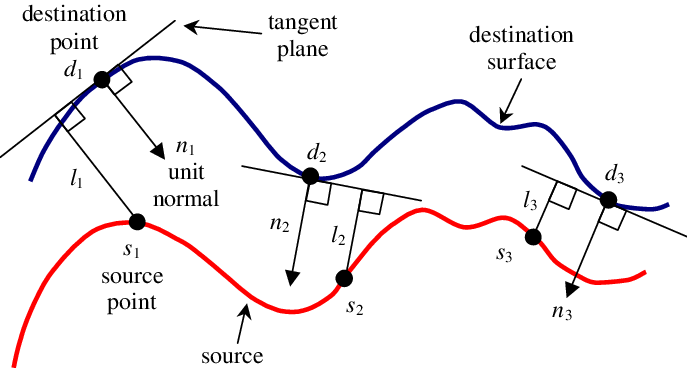
\includegraphics[width=0.8\textwidth]{images/icp_point_to_plane.png}
    \caption{The point-to-plane metric illustrated, one of the data association techniques there are. Image extracted from \cite{icp_point_to_plane_Low}.}
    \label{fig:icp_point_to_plane}
\end{figure}

\paragraph{Point cloud alignment from known correspondences} Once there is a data association for the points in the source and target clouds, the aim is to align those clouds by minimizing an objective function. What comes from minimizing said function is a rotation matrix $R$ and a translation vector $t$ to be applied to source cloud X. As mentioned before, after aligning, point correspondences are computed again, until convergence is reached. The following paragraphs are dedicated to the theory behind this alignment. As it will be shown, aligning two point clouds with known correspondences has a direct and optimal solution that does not require an initial guess. Note: this section is based off the seminar in \cite{stachniss_known_data_association} and the original article \cite{least_squares_3D_point_sets_Arun}.

The set of points in target cloud Y is defined as $Y=\{\boldsymbol{y}_{1}, \boldsymbol{y}_{2}, ..., \boldsymbol{y}_{I}\}$\footnote{Note that points are bold because they are 3-celled vectors that hold the position in space, like $\boldsymbol{x}_{n} = \begin{bmatrix} x & y & z \end{bmatrix}^{T}$ in the case of a point in the source cloud.} and source cloud $X=\{\boldsymbol{x}_{1}, \boldsymbol{x}_{2}, ..., \boldsymbol{x}_{J}\}$. As mentioned, it's X that is transformed to Y's position, and not vice versa. Assume every point in X is associated with another one in Y, such that $C=\{(i, j)\}$. The objective function to minimize is the following

\begin{equation} \label{eq:reg_minfun_1}
    \min \sum_{(i, j) \in C}\left\|\boldsymbol{y}_{i}-R \boldsymbol{x}_{j}-\boldsymbol{t}\right\|^{2}
\end{equation}

To simplify notation, corresponding points in X and Y (defined by $C$) are reordered under the same index $n$, which yields the sets $\{\boldsymbol{x}_{n}\}$ and $\{\boldsymbol{y}_{n}\}$. That is, the correspondence in $\boldsymbol{x}_{1}$ is $\boldsymbol{y}_{1}$, for $\boldsymbol{x}_{2}$ it's $\boldsymbol{y}_{2}$ and so on. The rigid body transform to apply to X is $\overline{\boldsymbol{x}}_{n} = R \boldsymbol{x}_{n}-\boldsymbol{t}$ for $n=1, ... \|C\|$. The transformed set of points $\{\overline{\boldsymbol{x}}_{n}\}$ will be as close as possible to the target cloud's point set $\{\boldsymbol{y}_{n}\}$, that is, having the minimum sum of squared point-to-point distances. Additionally, pairs of matching points may be weighted by $p_{n}$, indicating more or less correspondence importance due to certain factors, like distance. Hence, the objective function to be minimized in \ref{eq:reg_minfun_1} takes the following form

\begin{equation} \label{eq:reg_minfun_2}
    \min \sum\left\|\boldsymbol{y}_{n}-\overline{\boldsymbol{x}}_{n}\right\|^{2} p_{n} = \min \sum\left\|\boldsymbol{y}_{n} - R \boldsymbol{x}_{n}-\boldsymbol{t} \right\|^{2} p_{n}
\end{equation}

The first thing to do is to define a coordinate system. The coordinate system will be the target cloud Y, that is, the local coordinate defined by the set $\{y_{n}\}$. Said local coordinate will be the center of mass of $\{y_{n}\}$, computed by the weighted mean for all points, like

\begin{equation}
    \boldsymbol{y}_{0}=\frac{\sum \boldsymbol{y}_{n} p_{n}}{\sum p_{n}}
\end{equation}

This way, by centering all point sat this local coordinate $\boldsymbol{y}_{0}$, equation \ref{eq:reg_minfun_2} becomes

\begin{equation} \label{eq:reg_minfun_3}
    \min \sum\left\|\boldsymbol{y}_{n}-\boldsymbol{y}_{0}-\boldsymbol{R} \boldsymbol{x}_{n}-\boldsymbol{t}+\boldsymbol{y}_{0}\right\|^{2} p_{n} 
\end{equation}

The second thing to do is to shift $\overline{\boldsymbol{x}}_{n} = R \boldsymbol{x}_{n}-\boldsymbol{t}$ to the origin of the new local coordinate system, like so

\begin{equation}
    \overline{\boldsymbol{x}}_{n}-\boldsymbol{y}_{0}=R \boldsymbol{x}_{n}-\boldsymbol{t} - \boldsymbol{y}_{0}
\end{equation}

Rearranging the former equation, so that the rotation matrix $R$ multiplies the entire left hand side, one can obtain:

\begin{equation} 
    \overline{\boldsymbol{x}}_{n}-\boldsymbol{y}_{0}=R\left(\boldsymbol{x}_{n}+R^{\top} \boldsymbol{t}-R^{\top} \boldsymbol{y}_{0}\right)
\end{equation}

The reason behind this rearrangement is that it is convenient to rewrite the translation vector $t$ into something else. This will be a new vector, $\boldsymbol{x}_{0}=R^{\top} \boldsymbol{t}-R^{\top} \boldsymbol{y}_{0}$ (which, again, is unknown at the moment), that is summed to $\boldsymbol{x}_{n}$ and then rotated. Doing this will be useful later. Last equation will look like

\begin{equation} 
    \overline{\boldsymbol{x}}_{n}-\boldsymbol{y}_{0}=R\left(\boldsymbol{x}_{n}-\boldsymbol{x}_{0}\right)
\end{equation}

Last rearrangement leaves equation \ref{eq:reg_minfun_3} like the following

\begin{equation}
    \min \sum\left\|\boldsymbol{y}_{n}-\boldsymbol{y}_{0}-R\left(\boldsymbol{x}_{n}-\boldsymbol{x}_{0}\right)\right\|^{2} p_{n}
\end{equation}

where the aim to find $R$ and $\boldsymbol{x}_{0}$ that produce the function's minimum. Let's rearrange, again, last function for easier manipulation (the minimization function will be called $f(\boldsymbol{x}_{0}, R)$ from now on)

\begin{gather} %\label{eq:reg_minfun_4}
    f(\boldsymbol{x}_{0}, R) = \sum\left\|\boldsymbol{y}_{n}-\boldsymbol{y}_{0}-R\left(\boldsymbol{x}_{n}-\boldsymbol{x}_{0}\right)\right\|^{2} p_{n} = \nonumber \\
    = \sum\left[\left(\boldsymbol{y}_{n}-\boldsymbol{y}_{0}\right)-R\left(\boldsymbol{x}_{n}-\boldsymbol{x}_{0}\right)\right]^{\top} \left[\left(\boldsymbol{y}_{n}-\boldsymbol{y}_{0}\right)-R\left(\boldsymbol{x}_{n}-\boldsymbol{x}_{0}\right)\right] p_{n} = \nonumber \\
    = \sum\left(\boldsymbol{y}_{n}-\boldsymbol{y}_{0}\right)^{\top}\left(\boldsymbol{y}_{n}-\boldsymbol{y}_{0}\right) p_{n}+\sum\left(\boldsymbol{x}_{n}-\boldsymbol{x}_{0}\right)^{\top}\left(\boldsymbol{x}_{n}-\boldsymbol{x}_{0}\right) p_{n}-2 \sum\left(\boldsymbol{y}_{n}-\boldsymbol{y}_{0}\right)^{\top} R\left(\boldsymbol{x}_{n}-\boldsymbol{x}_{0}\right) p_{n} \label{eq:reg_minfun_4_separated}
\end{gather}

Note that, from the last equality, the first term does not depend on $\boldsymbol{x}_{0}$ nor $R$; the second term only depends on $\boldsymbol{x}_{0}$, and the third term depends on both. Minimizing $f(\boldsymbol{x}_{0}, R)$ requires differentiating and solving for $\frac{\partial f(\boldsymbol{x}_{0}, R)}{\partial \boldsymbol{x}_{0}}=0$, done below

\begin{equation}
    \frac{\partial f(\boldsymbol{x}_{0}, R)}{\partial \boldsymbol{x}_{0}}=-2 \sum\left(\boldsymbol{x}_{n}-\boldsymbol{x}_{0}\right) p_{n}+2 \sum R^{\top}\left(\boldsymbol{y}_{n}-\boldsymbol{y}_{0}\right) p_{n}=0
\end{equation}

This simplifies to 

\begin{equation}
    \sum\left(\boldsymbol{x}_{n}-\boldsymbol{x}_{0}\right) p_{n}=R^{\top} \sum\left(\boldsymbol{y}_{n}-\boldsymbol{y}_{0}\right) p_{n}
\end{equation}

However, it can be noted that $\sum\left(\boldsymbol{y}_{n}-\boldsymbol{y}_{0}\right) p_{n}=0$ since it is a summation of all points from the mean $\boldsymbol{y}_{0}$. This leaves $\sum\left(\boldsymbol{x}_{n}-\boldsymbol{x}_{0}\right) p_{n}=0$. Opening the parenthesis results in $\sum\boldsymbol{x}_{n}p_{n}-\boldsymbol{x}_{0}\sum p_{n}=0$ which, isolating for $\boldsymbol{x}_{0}$, is

\begin{equation}
    \boldsymbol{x}_{0}=\frac{\sum \boldsymbol{x}_{n} p_{n}}{\sum p_{n}}
\end{equation}

Which is the weighted mean of the set of points of cloud X. That is: the optimal value for $\boldsymbol{x}_{0}$ that minimizes the objective function is the weighted mean of $\{\boldsymbol{x}_{n}\}$. With $\boldsymbol{x}_{0}$ out of the way, now the optimal $R$ needs to be found. Looking at \ref{eq:reg_minfun_4_separated}, the only element that depends on $R$ is $-2 \sum\left(\boldsymbol{y}_{n}-\boldsymbol{y}_{0}\right)^{\top} R\left(\boldsymbol{x}_{n}-\boldsymbol{x}_{0}\right) p_{n}$. The minimum of this function is actually the maximum getting rid of the minus. The multiplying $2$ can also be removed. Hence it results in the following

\begin{equation} \label{eq:reg_minfun_5_R}
\begin{split}
    R^{*} &= \argmax_{R} \sum\left(\boldsymbol{y}_{n}-\boldsymbol{y}_{0}\right)^{\top} R\left(\boldsymbol{x}_{n}-\boldsymbol{x}_{0}\right) p_{n} = \\
    &= \argmax_{R}\Tr\left(\sum R \left(\boldsymbol{x}_{n}-\boldsymbol{x}_{0}\right) \left(\boldsymbol{y}_{n}-\boldsymbol{y}_{0}\right)^{\top}\right) \\
    &= \argmax_{R}\Tr \left(RH\right)
\end{split}
\end{equation}

where $H$ is the cross covariance matrix of both point clouds to register. To find what R maximizes the expression in \ref{eq:reg_minfun_5_R} the Singular Value Decomposition (SVD) is used. The SVD of the cross covariance $H$ is performed, which decomposes it in three matrices $U$, $D$, $V^{\top}$, like $H=UDV^{\top}$. $U$ is orthonormal and represents a rotation, $D$ is a stretch, and $V^{\top}$ is orthonormal and a rotation again. As properties of the SVD indicate, $U^{\top}U=I$, $V^{\top}V=I$ and $D$ is diagonal, and all matrices are $3 \times 3$. 

\begin{equation} \label{eq:reg_minfun_6_R}
\begin{split}
    R^{*}&= \argmax_{R}\Tr \left(RH\right)\\
    &= \argmax_{R}\Tr \left(RUDV^{\top}\right)
\end{split}
\end{equation}

As \cite{least_squares_3D_point_sets_Arun} indicates, a guess for $R$ could be $R=VU^{\top}$. In other words, \emph{what if} $R$ is made up of the two rotations obtained by the SVD of $H$? Would that be an optimal choice? Let's put that to the test

\begin{equation} \label{eq:tr_RH}
    \Tr \left(RH\right) = \Tr \left(VU^{\top}UDV^{\top}\right) = \Tr \left(VDV^{\top}\right)
\end{equation}

Is $\Tr \left(VDV^{\top}\right)$ maximal? It is, and that is demonstrated with the Schwarz inequality. Take $\Tr \left(VD^{\frac{1}{2}}\left(D^{\frac{1}{2}}V\right)^{\top}\right) \equiv \Tr\left(AA^{\top}\right)$, being $A=VD^{\frac{1}{2}}$ a positive definite matrix. The Schwarz inequality states that $\Tr\left(AA^{\top}\right) \geq \Tr\left(R'AA^{\top}\right)$ for any rotation matrix $R'$. In others words, $\Tr\left(RH\right) \geq \Tr\left(R'RH\right)$. That is, no other $R$ can make the trace larger than $R=VU^{\top}$ does, and hence it is the optimal one that maximizes \ref{eq:reg_minfun_6_R}.



\paragraph{Registration on the testbench using PCL} In the previous paragraphs the theory behind the composition of point cloud scenes has been explained. This section now presents the registration of several partial scenes taken from the testbench. 

PCL offers an entire API for registration, including variants of the baseline ICP, sampling methods, and data association methods. This thesis has used the simplest configuration, since it has been proven to suffice. That is: the standard Iterative Closest Point algorithm, uniform sampling and closest point association.



\subsection{Sample Consensus (SAC) segmentation} \label{sec:sac_segmentation}

\subsection{Euclidean Cluster segmentation} \label{sec:euclidean_segmentation}

\subsection{Region Growing segmentation} \label{sec:regiongrowing_segmentation}

% Local descriptors
\subsection{Local descriptor matching: the SHOT descriptor}

\subsection{Correspondence Grouping}





\end{document}